\documentclass[tikz]{standalone}
\newcommand{\vect}{\bm}
\newcommand{\Rearth}{R_e}
\newcommand{\lat}{\theta}
\newcommand{\lon}{\lambda}
\newcommand{\transpose}{\intercal}
\newcommand{\sign}{\mathrm{sgn}}
\newcommand{\unitlon}{\bm{\hat{\lon}}}
\newcommand{\unitlat}{\bm{\hat{\lat}}}
\newcommand{\unitk}{\bm{\hat{k}}}
\newcommand{\unitradius}{\bm{\hat{r}}}
\newcommand{\Mag}[1]{\left\lvert #1 \right\rvert}

\begin{document}
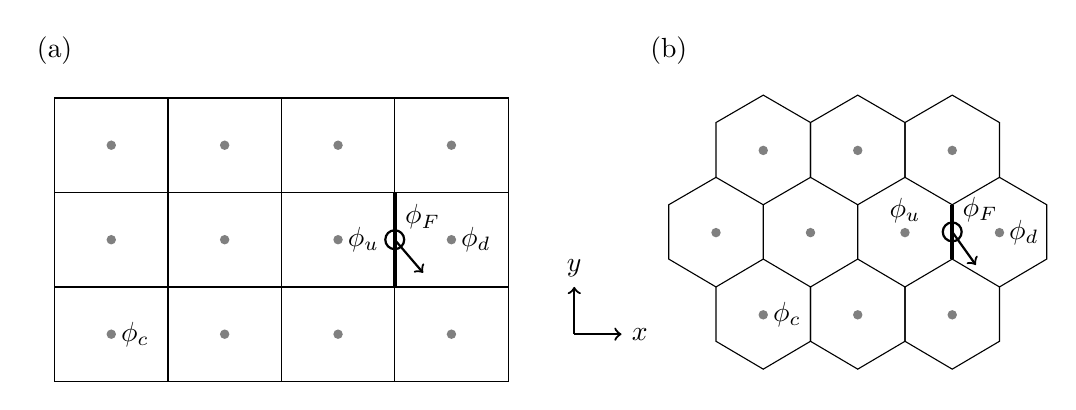
\begin{tikzpicture}[
  scale=0.6,
  cpnt/.style={fill=gray},
]

\begin{scope}[shift={(11,0)}]
	\draw [thick, ->] (0,1) -- (0,2) node [at end, anchor=south] {$y$};
	\draw [thick, ->] (0,1) -- (1,1) node [at end, anchor=west] {$x$};
\end{scope}

\node [above] at (0,6.5) {(a)};
\draw (0,0) rectangle (9.6,6);
\draw (0,2) -- (9.6,2);
\draw (0,4) -- (9.6,4);
\draw (0,0) -- (0,6);
\draw (2.4,0) -- (2.4,6);
\draw (4.8,0) -- (4.8,6);
\draw (7.2,0) -- (7.2,6);

\draw [ultra thick] (7.2,2) -- (7.2,4);
\draw [thick] (7.2,3) circle [radius=0.2] node [anchor=south west] {$\phi_F$};
\draw [thick, ->] (7.2,3) -- (7.8,2.3) node [anchor=west] {$\uf$};

\path [cpnt] (1.2,1) circle [radius=0.1] node [right] {$\phi_c$};
\path [cpnt] (1.2,3) circle [radius=0.1];
\path [cpnt] (1.2,5) circle [radius=0.1];

\path [cpnt] (3.6,1) circle [radius=0.1];
\path [cpnt] (3.6,3) circle [radius=0.1];
\path [cpnt] (3.6,5) circle [radius=0.1];

\path [cpnt] (6.0,1) circle [radius=0.1];
\path [cpnt] (6.0,3) circle [radius=0.1] node [right] {$\phi_u$};
\path [cpnt] (6.0,5) circle [radius=0.1];

\path [cpnt] (8.4,1) circle [radius=0.1];
\path [cpnt] (8.4,3) circle [radius=0.1] node [right] {$\phi_d$};
\path [cpnt] (8.4,5) circle [radius=0.1];

\begin{scope}[shift={(13,2)}]
	\node [above] at (0,4.5) {(b)};

	\draw (1,0) -- (0,0.59) -- (0,1.74) -- (1,2.32) -- (2,1.74) -- (2,0.59) -- (1,0); \path [cpnt] (1,1.15) circle [radius=0.1];
	\draw (2,1.74) -- (3,2.32) -- (4,1.74) -- (4,0.59) -- (3,0) -- (2,0.59); \path [cpnt] (3,1.15) circle [radius=0.1];
	\draw (4,1.74) -- (5,2.32) -- (6,1.74) -- (6,0.59) -- (5,0) -- (4,0.59); \path [cpnt] (5,1.15) circle [radius=0.1] node [above] {$\phi_u$};
	\draw (6,1.74) -- (7,2.32) -- (8,1.74) -- (8,0.59) -- (7,0) -- (6,0.59); \path [cpnt] (7,1.15) circle [radius=0.1] node [right] {$\phi_d$};

	\begin{scope}[shift={(1,-1.74)}]\draw (2,1.74) --(2,0.59) -- (1,0) -- (0,0.59) -- (0,1.74); \path [cpnt] (1,1.15) circle [radius=0.1] node [right] {$\phi_c$};\end{scope}
	\begin{scope}[shift={(3,-1.74)}]\draw (2,1.74) --(2,0.59) -- (1,0) -- (0,0.59) -- (0,1.74); \path [cpnt] (1,1.15) circle [radius=0.1];\end{scope}
	\begin{scope}[shift={(5,-1.74)}]\draw (2,1.74) --(2,0.59) -- (1,0) -- (0,0.59) -- (0,1.74); \path [cpnt] (1,1.15) circle [radius=0.1];\end{scope}

	\begin{scope}[shift={(1,1.74)}]\draw (0,0.59) -- (0,1.74) -- (1,2.32) -- (2,1.74) -- (2,0.59); \path [cpnt] (1,1.15) circle [radius=0.1];\end{scope}
	\begin{scope}[shift={(3,1.74)}]\draw (0,0.59) -- (0,1.74) -- (1,2.32) -- (2,1.74) -- (2,0.59); \path [cpnt] (1,1.15) circle [radius=0.1];\end{scope}
	\begin{scope}[shift={(5,1.74)}]\draw (0,0.59) -- (0,1.74) -- (1,2.32) -- (2,1.74) -- (2,0.59); \path [cpnt] (1,1.15) circle [radius=0.1];\end{scope}

	\draw [ultra thick] (6,0.59) -- (6,1.74);
	\draw [thick] (6,1.165) circle [radius=0.2] node [anchor=south west] {$\phi_F$};
	\draw [thick, ->] (6,1.165) -- (6.5,0.465) node [anchor=west] {$\uf$};
\end{scope}

\end{tikzpicture}
\end{document}
